\chapter[Bidding]{Prices and Bidding}
\label{appendix-bid-price}
\epigraph{One of the very important components in the urban and agricultural land use model is the so-called \gls{bid-rent curve}. Regional and urban economists, city planners, and economic geographers have used this curve extensively as an analytical device.}{Yeung-Nan Shieh\cite{shiehWilhelmLaunhardtBidRent2004}}

This chapter links the theoretical discussions of the previous chapters with an agent-based simulation model. At the heart of the model is a real estate market in which owners, tenants, new entrants to the city and non-resident investors participate. We need to specify the market process in more detail. To do that we build up our model in a series of steps beginning with a notion of economic value, adding potential speculative gains, and finally describing a transaction process. 

\section{Rent} \label{section-housing-price}



\subsection{Warranted Rent}
The warranted price for a given property, reflects the underlying economic value. In each period a house offer two kinds of services:  \gls{locational services}, access to the central city job and \gls{home services} proper.  

\subsubsection{Locational services}
Since people live in homes inside or outside the city, it's a share of the subsistence wage,  OWNERS CAN ALSO CAPTURE? Maybe move some of the discussion here.

Locational services are, on an annual basis, the rent premium, $w$, minus the transportation costs, $c$, for a property a given distance, $d$, from the center:
\[\omega- {dc}.\]

\subsubsection{Home services}
Home services proper includes the value of living in a house: a place to sleep, to prepare food, the amenity of being in the home, etc. Since people require housing inside and outside the city, home services are modeled as paid for as a share of the subsistence wage ($a \psi$). 



ADD A FOOTNOTE ABOUT THE DISTINCTION BETWEEN THE VALUE AND THE VALUE PAID? % - if you own the services you capture it - the value experienced can differ from the value paid. *** WORK OUT NOTATION AMENITY HERE OT MAKE IT EASIER LATER.. 
% MAYBE NOTE THEY STILL NEED TO PAY $a\psi$ OUTSIDE THE CITY. SO THAT'S THE CONSTANT
, so the warranted rent, $\mathcal{R}_W$, the maximum rent that is economically justified is:
% a property at $d$ offers the 

\subsubsection{Economically warranted rent}
The warranted rent is then the sum of the locational services and home services.
We call the value of this stream of services the \glspl{warranted rent}, $\mathcal{R}_W$, since it is the market value of the services provided. This is the maximum a tenant might pay, since it is the maximum that could be extracted from tenants before they decide they are better off leaving the city.
\begin{align}
\mathcal{R}_W=\omega- {dc} + a\psi.
\label{eqn-housing-price}
\end{align}

It is the combined annual services a property, at a distance $d$, offers to a worker in the city. It is thus the maximum that they may be charged.

NOTE ON AMENITY..

The price analysis that follows assumes that the actual market rental price is the warranted rental price. Rents can diverge from warranted rents. In practice, some people may pay more or less than the warranted rent. They may draw on family assets, assume debt, spend more on amenity, etc. Rents are, however, limited by what tenants can pay, and that, in turn, is limited by urban wages. 

Building this relationship into the model is a core conceptual contribution of this work. It makes it possible to explore formally the relationship between the scaling of urban productivity, and the potential for financialized ownership to extract that value, pushing those who contribute to creating growing wealth, to a subsistence frontier\footnote{***WHERE IS MAIN DISCUSSION OF THIS? %METHOD/model/intro section - ref section
COULD ELABORATE ON BENEFITS. THIS IS A CORE CONTRIBUTION, WE ARGUE IT IS QUITE WORTHWHILE TO EXPLORE THE LINKAGES BETWEEN PRODUCTION AND EXTRACTION. TO OUR KNOWLEDGE, IT HAS NOT BEEN DONE ELSEWHERE. Future work can explore the way in which this locks those who earn bellow average incomes to fall behind, no matter how much wealth they create, the smaller urban concentration of value may increase the total value produced, but also makes it easier to monopolize land and concentrate in a financialized ownership class, that amplifies whatever advantage it begins with, however small or path dependant, (shared ownership is in a sense an unstable equilibrium, under the conditions of combining urban scaling laws and a land tenure models that allows finacialization)  REFERENCE HERE AND  MOVE/EXPAND DISCUSSION IN FUTURE WORK}.

The warranted rent %is a frontier the market pushes the agents towards.  
is a kind of frontier, which may be thought of as an equilibrium or attractor. The way this work uses that kind of frontier, drawing on equilibrium, dynamical system, and agent-based traditions of analysis, is treated in detail in the discussion of methodology in Chapter \ref{chapter-methodology}.

Making this assumption simplifies the model and, along with the focus on rents, is what makes this a ``classical'' model.  When we assume an subsistence wage $\psi$ with a specific share $a$ applied to housing we are implicitly assuming that tenants are squeezed as much as possible by landlords. This is the way classical economists employed the subsistence wage assumption to simplify their analysis. 

% \subsubsection{Land and building services}
% Annual rent charged initially should be  equal to the annual value of services, $h$:
% and the warranted price is 
% \[P_W=\frac{\omega- {c} * d + a\psi}{r}\]

% We will use this value as the price for the first period 
% $P_W=\frac{\omega- {c} * d + a\psi}{r}$

\subsubsection{Net Rent}
Warranted rent defines what agents would pay to live in a property. Net rent is the warranted rent net of costs. Homes must be maintained and taxes paid, so an owner would claim not the total warranted rent, but the net rent after expenses,

\begin{align}
\mathcal{R}_N &= \mathcal{R}_W - \mathcal{O} - \mathcal{T}\\
&= \omega - {dc} + a\psi -  \mathcal{O} - \mathcal{T}, \\
\end{align}
where $\mathcal{O}$ is operating costs and  $\mathcal{T}$ taxes.   $\mathcal{R}_N$ is the maximum it's worth paying to get the capture the return on a property, so it is the value that investors when assessing the \gls{financial return} on an investment.
consider in investment decisions. % of services and costs


When considering the , 

For an investor, it is $\mathcal{R}_N$  that is relevant in investment decisions. % ( - fees, cost of money etc.) decision making. 

\subsection{Market Rent}
The market rent is what the investor actually pays for the property.

ADD DISTINCTION BETWEEN REALIZED MARKET RENT AND DIFFERENT KINDS OF EXPECTATIONS --- THEY WONT ACTUALLY BE THE PREDICTION VALUES. THE PREDICTION VALUES ARE WHAT ARE USED. 
THEY PREDICTION VALUES CAN INCLUDE ERRORS, BIASES, ETC.
WE USE THE EQUILIBRIUM TO EXPLORE A SET OF FRONTIERS RIGOROUSLY.

\subsection{Annual Taxation}
In each  period a `mill rate' is applied to the assessed value. For computational purposes, we will assume that, that is the warranted price.  Municipal taxes are based on the appraised value, which is based, somewhat approximately and with a lag. The warranted price,  Equation \ref{eqn-price-warranted}.
\[P_W = \frac{\omega- {dc} + a\psi}{r}.\]
% value of the stream of services.. why 
Since the appraised value typically lags the market value, and attempts to approximate underlying value, it is reasonable to approximated it with the warranted price \cite{apraised_value_refs}.

Each mill is expressed as  1/1,000 of the value as determine by assessment \footnote{By capitalizing the mill rate at 5\%  we see that each `mill' is worth about 2\% of the warranted rents. Assessments usually understate the market value considerably. Mill rates are commonly about 1.5 and differ between municipalities. ***MAYBE MOVE PARAM VALUES TO PARAM DISCUSSION}. The annual tax is then:
\begin{align*}
\mathcal{T} &= \text{mill rate} \times \frac{\mathcal{R}_N}{r} \\
 *** FIX &= \text{mill rate} \times \frac{\omega- {dc} + a\psi}{r}
\end{align*}

The net rent is the one that's used in the financial assessment, and thus in price and bidding decisions, and so it is the value used in tax assessments, as tax assessments are based loosely -- on the market price. 

In our computations, the rate selected has to be compounded for decisions made over a period of the mortgage term $T$.

\subsubsection{Annual Maintenance}
Annual maintenance costs apply to building and lands but not to locational value.

% \subsection{Distinguishing net market rental price and warranted rent}
% Why? A tenant should expect to pay a market price for the combination of locational services and the services of land and buildings that they use.  The market rental price  is an equilibrium market rent, not the economic economic rent. In the real world the market rental price can  diverge from the warranted . )  
WE MAY  WANT A TERM FOR EQUILIBRIUM MARKET PRICE, TO DISTINGUISH IT FROM THE EVOLVED MARKET PRICE  % LIKE MARKET PRICE, IT IS THE PRODUCT OF A DISTINCT PROCESS OFMARKET EVOLUTION. THAT WOULD LET US TALK ABOUT THESE TWO KINDS OF MARKETS WE ARE LOOKING AT (E CONFUSES IT WITH EXPECTEED THOUGH.. 
MAYBE USE $\epsilon$ FOR EXPECTED SUPERSCRIPT e.g. $P_M^{\epsilon}$? % THEN IT IS THE EXPECTATION OF A PARTICULAR AGENT, WHICH CAN DIVERGE FROM EQULIBRIUM-- IT CAN HAVE ANY GUESSES OR SPECULATION ABOUT OTHER AGENTS THAT WE WANT TO ADD--
 $P_M^{E}$ is the equilibrium expectation based on precisely articulated assumptions, either rational expectations or another set of explicitly stated rules,  $P_M^{\epsilon}$ is an agent's expectation. The agent's expectation can include any assumptions the agent has about the behaviour of others, the system state, etc. % Neither is a true realized value. This probably confuses things to carry 

% We should distinguish the locational rent from the $\mathcal{R}^l = \omega - {dc}$ from the warranted rental cost of housing services.% (Maybe use a capital L?) 

% Market  rental price $\mathcal{R}^w$ should  include the services of the house and land.  $\mathcal{R}^w =\mathcal{R}^l+\mathcal{R}^h$ 

% \begin{quotation}
% a  =  share of subsistence wage  used for land and building e.g. 0.3

% b  = share of share of subsistence wage  used on maintenance e.g. 0.2

% c  = annual tax rate on rent and home  e.g. 12 mills = 0.012
% \end{quotation}

% Now the net  market rental price is


% It is also net warranted  rental price that is relevant in taxation and maintenance. 

\begin{align}
\mathcal{O} &\equiv  ba\psi\\%Maintenance?
 \mathcal{T} &\equiv c(\omega-{dc}+a\psi) %taxes?
\end{align}
so we can write
 \begin{align}
\mathcal{R}_N^w &= \omega - {dc}  + a\psi -   ba\psi - c(\omega-{dc}+a\psi) \\
\end{align}

% All of these are in annual values. We will use the present values  for the appropriate period  T in computations. (See notes on the present value calculations to use)

% \subsection{NEW WORK STARTS - How does this affect the bid price?}

% I now return to Equations B6 to compute the value of a proposed purchase


% \begin{align*}
% V &= \delta \left(P_T - (1+r)M\right) +      \mathcal{R}^w_N  \tag{B6} \\
%   &= \delta \left((1+\dot P)    - (1+r)m    \right) P_B + \mathcal{R}^w_N%\label{eqn-property-investment-value1}
% \end{align*}
% Similarly, Equation B7 becomes

% \begin{align*}
% r_{return} = \frac{\delta \left(1 + \dot P - (1+r)m\right)}{1-m} + \frac{\mathcal{R}^w_N}{(1-m)^{bid}}\tag{B7}
% \end{align*}
% And following the same sequence of steps to derive the bid price 

% \begin{align*}
% P_i^{bid} \le &   \frac{\mathcal{R}^w_N}{(1-m_i)r_i^{target} - \delta_i \left(1 + L(P) - (1+r_i)m_i \right)} \tag{B10}\\
% 		 \le &   \frac{ \omega - dc + a\psi -   ba\psi - ca\psi}{(1-m_i)r_i^{target} - \delta_i \left(1 + L(P) - (1+r_i)m_i \right)}	\\	
%    		 \le &   \frac{ \omega - dc + a(1-b-c)\psi}{(1-m_i)r_i^{target} - \delta_i \left(1 + L(P) - (1+r_i)m_i \right)}	
% \end{align*}

%Our conclusion about the advantage that the bank and the wealthy have can be read out of this equation. 
%That may let us simplify the exposition in the financialization chapter.

\subsubsection{Warranted price}

The \gls{warranted price} of a house is the present discounted value of the flow of service net of costs:
\begin{equation}
  P_W=\frac{\mathcal{R}_N}{r},  
\label{eqn-price-warranted}
\end{equation}
where $\mathcal{R}_N$ is the net value of rents, and $r$ is the interest rate.  The warranted price approximates the sale price, of a unit of housing with land, in the absence of potential capital gains. 


\section{Bid Price}

The warranted price is not the same as the market price.  The market price can depart from the warranted price when there is price speculation based on expected future values or if agents make errors based on market information.
% There is another distinction:
The warranted value is base on the true value of the services, while the market value can diverge. 
% We do the calculation in terms of warranted values because we will use these to initialize the model. 

The actual market price will be determined by a bidding process that takes into account potential capital gains.  We describe the bid price formulation below. % that process below.

For the sake of the computational model we define housing prices for different purposes and at different stages of the market process. The notation appears in Table \ref{table-price-notation}.

*** TABLE ALSO NEEDS NET RENT $\mathcal{R}_N$ - WE SHOULD THINK ABOUT BEST WAY TO COMMUNICATE RELATIONSHIPS BETWEEN RENT TERMS.
\begin{table}[]
\centering
\begin{tabular}{r|c|c|c|c|c|c|}\cline{2-7}
                     & Warranted       & Asking  & Bid  & Reservation & Market          & Expected \\ \cline{2-7}
Property price       & $P_W$           & $P_A$  & $P_B$ & $P_R$       & $P_M$           & $P_M^e$  \\ \cline{2-7}
Rent $\mathcal{R}_W$ & $\mathcal{R}_W$ &        &       &             & $\mathcal{R}_M$ &          \\ \cline{2-7}
\end{tabular}
\caption{Price and rent notation}
\label{table-price-notation}
\end{table}

% \renewcommand{\arraystretch}{1.5}
% \begin{tabular}{rlrr}\
% Symbol         & Name                                 & Value      & Formula  \\ \hline
% $\omega$  & Maximum locational rent (wage premium) & 0.012  \\
% $a$       & Share of subsistence wage for land and building & 1.0 \\
% $\psi$    & Subsistence wage & 10000 \\
% $tau$ replace  & Property tax rate &  e.g 1.6\% = 16 mills             & \\
% $c$       & Transportation cost & \\
% $T$       & Period & 5 years      \\
% $r$       & Individual interest rate & 0.05 \\\
% $\tau$       & Tax share & \\

% --        &  & \\
% $\dot P $      & Price growth                         & []         & $\frac{P_t-P_{t-1}}{P_{t-1}}$\\
% % $P^T_e$        & Expected price in T years            &            & $P_0(1+\dot P)^T$ \\ % *** WAS $P^e_T$ 
% $r_i^\delta$   & Individual discount rate             &            & To assign \\
% $\bar r$       & Prime interest rate                  &            & \\
% \end{tabular}
% \renewcommand{\arraystretch}{1.0}

We anchor our housing price expectations in bid rents, which, based on the literature can reasonably be seen as an equilibrium or attractor towards which prices will evolve. 

To model the market transactions when speculative motives are in play we need an expression for how much financial investors will bid. More specifically, we need to find the maximum price that they are willing to pay. As Horowitz \cite{horowitzBiddingModelsHousing1986} notes, a prospective buyer  considering knows a vector of attributes of the house, the seller’s asking price and the property taxes, transaction costs, and financing costs at a specified price. The  potential buyer also is likely to have estimates of the maintenance costs and resale value of the house, although these may be highly subjective. For our bidding model, therefore, we need find how much financial investors will bid in terms of these variables.

 We assume that agent may be  speculating on potential \glspl{capital gain} as well as on the \gls{use value} or net market rent they get from the property. We therefore treat the purchase as an investment decision and compute a rate of return, $v$, conditional on the price paid. This allows us to solve for the maximum bid, $P_{max}^{bid}$ that achieves the desired rate of return. 
    
 The agent purchases makes a down payment, $D$ on a house for a price, $P_0$, and agrees to payoff a mortgage with interest at the end of the mortgage period. For expositional convenience we can treat the mortgage period $T$ as a single term and express all quantities  in present-value terms. The Agent 
 and receives the increased price $P_T = (1 + \dot P)P_0$, back after a period $T$, Where $\dot P$ is the expected rate of price increase. The agent also receives either the net market rental value of the property, $\mathcal{R}^w_N$, or if the owner is also the resident, the locational rents.

 \subsection{The value of an investment}
The value of the investment $V$ is therefore the capital gain, minus financing costs, plus the rents, net of operating costs and taxes, $\mathcal{R}_N$.
 
 This may be written in terms of the purchase price, and several individual parameters: interest  rate, share of the price that can be mortgaged and  discount rate:\footnote{The down payment could be deducted in advance, but if the discount rate is equal to the interest rate it drops out completely.}
 
\begin{align}
V &= \delta \left(P_T - (1+r)M\right) +   \mathcal{R}^w_N   \\
&= \delta \left((1+\dot P) P_0 - (1+r)mP_0\right)  +      \mathcal{R}^w_N \\
%V &=& \delta \left(P_T - (1+r)M\right) +  \mathcal{R}^w_N\\
  &= \delta \left((1+\dot P)    - (1+r)m    \right) P_0 + \mathcal{R}^w_N 
\end{align}

This is the net present value of buying, and selling after one planning period. All rates are scaled to the length of the period to avoid the need for compounding calculations. The has 4 individualized  parameters, $\delta$, $\dot p$, $r$, $m$, as well as any factors that affect the rent term.



\subsection{Rate of return on investment}
The rate of return on funds invested is V divided by the size of the down payment, $D$ to get the rate of return  

\begin{align}
r^{return} 
  &= \frac{V}{D}  \nonumber \\
  &= \left(\delta \left(1+\dot P - (1+r)m\right) \ \right) \frac{P_0}{D}  + \frac{\mathcal{R}^w_N }{D}      \nonumber \\
  &= \left(\delta \left(1+\dot P - (1+r)m\right)  \right) \frac{P_0}{P_0-mP_0} +  \frac{\mathcal{R}^w_N }{P_0-mP_0}  \\ 
  &= \frac{\delta \left(1+\dot P - (1+r)m\right) }{1-m} +\frac{\mathcal{R}^w_N }{(1-m)P_0}.
\label{eqn-property-investment-return1}
\end{align}

\subsection{Criterion for investment}
Equation~\ref{eqn-property-investment-return1} provides a criterion for investors. Agents invest if if their expected return is greater than the target return, they are seeking:
\begin{equation}\Large
r^{target}\le v 
\label{eqn-property-investment-return2}
\end{equation}

% So the condition is 
% \begin{align*}
% r^{target} \le \frac{\delta \left(1 + \dot P - (1+r)m\right)}{1-m} + \frac{\mathcal{R}^w_N}{(1-m)P_0^{bid}}\tag{B7}
% \end{align*}

 % THIS  MAY BE NEEDED
% \begin{align*}
% P_{max}^{bid} \le &   \frac{\mathcal{R}^w_N}{(1-m_i)r_i^{target} - \delta_i \left(1 + L(P) - (1+r_i)m_i \right)} \tag{B10}\\
% 		 \le &   \frac{ \omega - dc + a\psi -   ba\psi - ca\psi}{(1-m_i)r_i^{target} - \delta_i \left(1 + L(P) - (1+r_i)m_i \right)}	\\	
%    		 \le &   \frac{ \omega - dc + a(1-b-c)\psi}{(1-m_i)r_i^{target} - \delta_i \left(1 + L(P) - (1+r_i)m_i \right)}	
% \end{align*}

 % We assume that the use value is captured by the stream of rental values. %, whether a home is owner-occupied or held by an investor as a financial asset. 
 % For simplicity, we consider a one-period investment.  %To keep the analysis simple without loss of generality 

%  The agent purchases a house for a price, $P_0$ %a down payment, $D$, 
%  and receives the increased price $P_T = (1 + \dot P)P_0$, back after a period $T$. 
% % The value of the investment is the net present value of buying and then selling after one period:
% The value of the investment is the capital gain, $\mathcal{C}$ plus the rents, net of operating costs and taxes, $\mathcal{R}_N$.

% minus the mortgage, repaid with interest, plus rents, minus any operating costs and taxes,\footnote{We have applied this model to explore the effect of a vacancy tax in Beirut.  For that analysis we  added a use-value, $U$ in place of rent for expatriate owners to represent using the property - say one month a year - when they are not renting the property and a \textbf{vacancy tax}, $T$ at rate $t$ to affect the speculator's  decision.} %\cite{Al-Shihabi}

% OLD equations from working out the above. Could change symbols
% \begin{eqnarray}
% V  	&=& capital\ gain - Interest\ due  	+ Rent  - operating\ cost -taxes \\
% 	&=& \delta P_T-D \qquad \qquad \quad - (1+\delta r)M \quad	 + R  	-C\\
% 	&=& \delta P _T \qquad-(P_0-M) \quad- (1+\delta r)M 	 + R  	-C\\
% 	&=& \delta (1+\dot P)  P_0 -(P_O -M)  -(1+\delta r)mP_0  + R  -C\\
% 	&=& \delta (1+\dot P)  P_0 -P_O + M \qquad -(1+\delta r)mP_0  + R -C\\
% 	&=&( \delta (1+\dot P)-1)  P_0  + mP_0 \quad -(1+ \delta r)mP_0  + (\rho-\kappa)P_0 \\	
% 	&=& \left(  \delta (1+\dot P)-1    + m \quad - m(1+\delta r)  + (\rho-\kappa)\right)P_0 \\'
% 	&=& \left(  \delta (1+\dot P)-1    + m \quad - m-\delta rm  + (\rho-\kappa)\right)P_0
% \end{eqnarray}
 % Where $\mathcal{R}$, $\mathcal{O}$, $\mathcal{T}$, and $M$ are total rent, operating costs, tax payments, and mortgage borrowed, as net present values at the end of the period. The interest rate is $r$, and the discount factor $\delta$. % I don't like this. I think it makes sense for them to be total payments over the period, but I now think it would be more intuitive to compute them as net present values at the start of the period, since that is when the mortgage is borrowed and the decision is made.

 %For ease of calculation, ..To get the return on investment, 
%  This may be written in terms of shares of the purchase price:
% \begin{eqnarray}
% V &=& \delta \left((1+\dot P) P_0 - (1+r)mP_0\right) + \rho P_0 - \theta P_0 - \tau P_0 \nonumber \\
%   &=& \left(\delta \left(1+\dot P - (1+r)m   \right) + \rho     - \theta     - \tau\right) P_0.
% \label{eqn-property-investment-value2}
% \end{eqnarray}
%  Where $\rho$, $\theta$, $\tau$, and $m$ are rent, operating costs, taxes, and mortgage shares, respectively. % Where $\phi$ is a fraction that takes into account taxes and operating costs. 
 % of price for rents, operating costs, and taxes. %The discount factor is $delta$, $P_0$ is the property price at the time of sale. %$r$ is the interest rate paid, and $m$ is the share of the price taken out as a mortgage.
 %It has  seven  parameters, $\delta, \dot P, r, m, \rho, \kappa$ and $t$. The first four, $\delta, \dot P, r$ and $m$ are exogenous for the investor while $\rho$, $\kappa$ and $t$  are    %Operating revenue and costs $\rho, \kappa$ and $t$ are expressed as  present values. 

%Agents borrow a share of the purchase price, $P$. The amount borrowed is the mortgage, $M$. This is a share of the total purchase price $mP = M$. The \gls{mortgage term}, $T$, is the period it takes to pay down the mortgage.

%\section{Return on investment}

% The rate of return on funds invested, $r_{return}$, is the value divided by the size of the down payment, $D$: 
% %The rate of return is $v = \frac{V}{D}$. %For expat investors, we get a \textbf{decision rule}:
% %\begin{enumerate}
% %\item  if $v \geq a$ (with some private use?) with no rent,  don't bother renting. 
% %\item If $v(no\ rent\ and\ tax) < a\geq v(with\ rent)$,  then  rent. 
% %\item If $ v(with\ rent) \le a $,  then sell 
% %\end{enumerate}\
% \begin{eqnarray}
% r^{return} 
%   &=& \frac{V}{D}  \nonumber \\
%   &=& \left(\delta \left(1+\dot P - (1+r)m\right) \ + \rho - \theta - \tau \right) \frac{P_0}{D}        \nonumber \\
%   &=& \left(\delta \left(1+\dot P - (1+r)m\right) \ + \rho - \theta - \tau \right) \frac{P_0}{P_0-mP_0} \nonumber \\ 
%   &=& \frac{\delta \left(1+\dot P - (1+r)m\right) \ + \rho - \theta - \tau }{1-m}.
% \label{eqn-property-investment-return1}
% \end{eqnarray}
% Equation~\ref{eqn-property-investment-return1} provides a criterion for investors. Agents invest if if their expected return is greater than the target return, they are seeking:
% \begin{equation}
% r^{return} \geq r^{target}. 
% \label{eqn-property-investment-return2}
% \end{equation}

%This is the maximum price that satisfies the criterion $r^{return} \geq r^{target}$.  The bid price is used in the price determination process in our model. %Where the return is the value over the down payment:
% Equation \ref{eqn-property-investment-return1} expresses the expected return on investment in terms of the  market price, $P_0$: 
% \begin{eqnarray*}
%  r^{return} 
%    &=& \frac{V}{D} \\
%    &=& \frac{\delta \left(1+\dot P - (1+r)m\right) \ + \rho - \theta - \tau}{1-m}.
% \end{eqnarray*}
%which we define as the ``bid price'',% $P_B$ $P^{max}_{bid}$. 
%We return to Equation~\ref{eqn-property-investment-value3} %
%We start by writing the value of the investment, from Equation \ref{eqn-property-investment-value1}, with the net rent. %, which can be written a share, $\phi$ of total rent $\mathcal{R}_N = \phi \mathcal{R}$, %The net rent can also be written as a share, $\phi$, of the rent 
%: %(originally from Chapter \ref{chapter-financialization} on Financialization. Since the rent is a known quantity at the beginning of the term, independent of the current, so we reformulate net rent,  $\mathcal{R}$, $\mathcal{O}$, $\mathcal{T}$ as a fraction of total rent: 

% \begin{eqnarray}
% V &=& \delta \left(P_T - (1+r)M\right) +      \mathcal{R}_N   \nonumber \\
%   % &=& \delta \left(P_T - (1+r)M\right) + \mathcal{R}_N   \nonumber \\
%   % &=& \delta \left(P_T - (1+r)m P_0\right) + \mathcal{R}_N \nonumber \\
%   &=& \delta \left((1+\dot P)P_0 - (1+r)m P_0\right)     + \mathcal{R}_N \nonumber \\
%   &=& \delta \left((1+\dot P)    - (1+r)m    \right) P_0 + \mathcal{R}_N
% \label{eqn-property-investment-value3}
% \end{eqnarray}


% Dividing by the down payment, $D = (1-m)P_0$:
% \begin{eqnarray}
% r_{return} = \frac{\delta \left(1 + \dot P - (1+r)m\right)}{1-m} + \frac{\mathcal{R}_N}{(1-m)P_0}
% \end{eqnarray}

% +++++++++++++++ JUST REPLACED BETWEEN THESE WITH THE ABOVE. CHECK IT'S OKAY
% % We also have to assume that $P_B = P_M$, which we can justify as an equilibrium condition - investors believe they are paying the market price. The result is 
% % \[V= \delta(P^T- (1+r)M)   +\phi r P_B\]

% % The price at the end of the term $T$, $P_T$, is a predicted value for the investor \textit{ex-ante}, so we can replace $P^T$ in Equation~\ref{eqn-property-investment-value3} with the predictor, $(1+\dot P)P_B$. 
% % We can replace $P^T$ in Equation~\ref{eqn-property-investment-value3} with $(1+\dot P)P_0$.
% \[V= \delta \left((1+\dot P)P_0 - (1+r)m P_0\right) +\phi \mathcal{R}\] 
% Then we replace $\dot P$ with an estimate, $L(P)$, representing an estimated function of the lagged values of $P$ and any  other relevant data. We imagine the potential investor informed estimates by information from  real estate agents or analysts.  The result is 
% \[V= \delta \left((1+L(P))P_B- (1+r)mP_B\right) +\phi \mathcal{R}\]
% Combining terms:
% \[V= \delta \left((1+L(P))- (1+r)m \right) P_B +\phi \mathcal{R}\]

% WHY BIG BRACKETS NOT SHOWING UP

% The rate of return $r_{return}=V/D=V/(1-m)P_B$ is then

% \[r_{return}= \frac{\delta \left((1+L(P) - (1+r)m\right)}{1-m} + \frac{\phi \mathcal{R}}{(1-m)P_B}\]

% %++++++++++++++++

% \begin{align}  
%   v  & =  \frac{\delta ((1+\dot P)  - (1+r)m)\  + \psi r}{1-m}\label{eq:RULE}\\
%   & =  \frac{\delta ((1+\dot P)  - (1+r)m)\  + \psi r}{1-m}\label{eq:RULE}
% \end{align}

% \begin{eqnarray}
% v %&=& \delta(P^T- (1+r)M) \qquad \qquad \qquad 	 + \mathcal{R}_N \nonumber\\
% % &=&\delta\left( (1+\dot P)P_B - (1+r)mP_B \right)  + \mathcal{R}_N  \nonumber\\
%   &=&\delta\left( (1+L(p)) - (1+r)m \right) P_B + \mathcal{R}_N  \nonumber
% \end{eqnarray}

\subsection{Maximum bid} % given the rate of return

Agents bid if the RHS is larger than the target rate of return, as stated in Equation \ref{eqn-property-investment-return2}.  $P_0$ with $P_B$, and $\dot P$ with an estimator for $\dot P$, we get: %TO DO REPLACE PDOT - MAYBE WITH TILDE AND DOT..: 

\begin{eqnarray}
r_{target} \le \frac{\delta \left((1+ \dot P_M^e - (1+r)m\right)}{1-m} + \frac{\mathcal{R}_N}{(1-m)P_B}
\end{eqnarray}

Solving for $P_{bid}$:

\begin{align}
r^{target} &\le \frac{\delta \left(1 + \dot P_M^e - (1+r)m\right)}{1-m}   +\frac{\mathcal{R}_N}{(1-m)P_B}. \nonumber \\
(1-m)r^{target} &\le \ \ \delta \left(1 + \dot P_M^e - (1+r)m\right) + \frac{\mathcal{R}_N}{P_B} \nonumber \\ %\delta(1+L(P))- (1+r)m%
(1-m)r^{target} - \delta \left(1 + \dot P_M^e - (1+r)m\right)  &\le  \frac{\mathcal{R}_N}{P_B} \nonumber\\
P_B & \le    \frac{\mathcal{R}_N}{(1-m)r^{target}-\delta \left(1 + \dot P_M^e - (1+r)m\right)} 
% P_B & \le    \frac{\mathcal{R}_N}{(1-m)r^{target}-\left[ \delta(1+L(P)- (1+r)m\right]} \nonumber 
\label{eqn-bid-price1}
\end{align}
The denominator is an adjusted rate of return for capitalizing net rents, analogous to the value of $r$ in Equation~\ref{eqn-price-warranted}. 

Each agent has their own interest rates, discount rates, mortgage share, information, and expectations, so individual bids can differ.

% \begin{align}
% P_i^{bid} \le   \frac{\mathcal{R}_N}{(1-m_i)r_i^{target} - \delta_i \left(1 + L(P) - (1+r_i)m_i \right)}.
% \label{eqn-bid-price2}
% \end{align}

% \begin{eqnarray}%. OLD VERSION: WRONG
% %r^{target}&=& \delta\left( (1+L(p)) - (1+r)m \right) P^{max}_{bid} + \mathcal{R}_N  \nonumber\\
%    P_{max_bid} &=&\frac{r^{target} - \mathcal{R}_N}{\delta\left((1+L(p)) - (1+r)m \right)} %\label{EqBidPrice2} 
% \end{eqnarray}

% \section{Finding bid price}
% We start with Equation~\ref{B2}. for convenience, replace $\rho -\kappa - \sigma $ with $\mathcal{R}_N$ (net Rent). 

% Replace $P^T$ with $(1+\dot P)P_B$ assuming that the bidder is bidding the equilibrium market price for the period.

% Then replace   $\dot P$ with $L(p)$ representing some (estimated function ($\tilde{\dot P}$)) of the lagged values of $P$ that incorporates other data. 

% \begin{eqnarray}
% v&=& \delta(P^T- (1+r)M) \qquad \qquad \qquad 	 + \mathcal{R}_N \nonumber\\
%  &=&\delta\left( (1+\dot P)P_B - (1+r)mP_B \right)  + \mathcal{R}_N  \nonumber\\
%   &=&\delta\left( (1+L(p)) - (1+r)m \right) P_B + \mathcal{R}_N  \nonumber
% \end{eqnarray}

% So I want to use this relationship to find the maximum bid price for the bank. The rule is, ``Bid if the RHS is larger than the target rate of return, $r^{target}$, and do not bid if it is smaller.''  The maximum bid  is the bid that makes the two sides equal. 

% {\color{red}
% \begin{eqnarray}
% r^{target}&=& \delta\left( (1+L(p)) - (1+r)m \right) P^{max}_{bid} + \mathcal{R}_N  \nonumber\\
%    P^{max}_{bid} &=&\frac{r^{target}-\mathcal{R}_N}{\delta\left( (1+L(p)) - (1+r)m \right)} \label{EqBidPrice} 
% \end{eqnarray}}
% %(What makes. this work is that I do not use an identity to get $\dot P$, which made the system of equations singular.)
% \newpage



\section{The period and time value of money}

In developing the model we introduced a number of rates, such as $r_i$, the rate that individual $i$ pays for a single borrowing period. The payment calculation is made for a period of length $T$, which we refer to as a mortgage term.
%This means the actual interest paid is a compounded interest rates (VARIABLES LIST FOR THIS).

%In developing the theoretical model we introduced a number of rates, such as $r_i$, the rate that  individual $i$ pays for a single period of borrowing. We assume the calculations are for a  period of length  $T$, which we refer to as a mortgage term. This means that the rates in equations such XXXXX are actually compounded rates.
Taking a simplified example, if the rate is $x$/year, interest payments are $xM$, a share of the total mortgage amount borrowed, $M$, for each of $T$ years. 
If the interest payments are all made at the end of the mortgage term, the lender will require interest on the deferred interest, so agent $i$'s payment at the end of the period $T$ will be:

\begin{align*}
\text{Payment} &= (1+r_i)M                                 \\ 
    &= M + xM(1+x)^{T-1}+ xM(1+x)^{T-2}\dots + xM(1+x)^{0} \\
    &= M\left(1+ x\sum_{z=T-1}^0(1+x)^{z}\right).          \\ 
\end{align*}
Therefore, the interest payment is:
\begin{align*}
r_i.   &=x\sum_{z=T-1}^0(1+x)^{z}.
\end{align*}

For the sake of notational simplicity and clarity of exposition,  we omit the compounding formula throughout our discussion. This means that, while banks may quote a per period interest rates, the equations use a compounded rate. In the computational model we employ the appropriately compounded values. All %the rates are compounded in this way to provide a per-period rates, including all 
 the interest rates, the $r$'s, are compounded in this way, because they require annual or monthly payments at their stated rates.
 It does not affect the discount rates, the $\delta$'s, or the borrowing ratio $m_i$, because they are initially calculated for the term and don't require the same period payments.
 The discount factor $\delta_i$ is always a compounded version of $x$:
 \[\delta_i=\left(\frac{1}{1+x}\right)^T\].
%is a feature of the individual, so it is not affected in this way.
%The appropriate compunding expressions for other rates are displayed below.

 The {mortgage term}, $T$, is the period after which the mortgage must be repaid with interest. We work with a mortgage terms for two reasons. First, in the theoretical analysis, by transforming the multi-period transaction to a single period, we simplify the comprehensibility of the analysis. Second, it reflects the fact that in practice agents  likely consider the profitability of a purchase for a finite term longer than one period. The term period lets them consider the time cost of money in their analysis in a natural way. Parameters for their discounting rates and the term considered can be used to explore the effect of borrowing costs and their personal discounting rates on their decisions. Future interest rates are also not fully known. In the future, we can also vary the compound interest rates to explore the impact of uncertainty, given agents' guesses about the future, and their level of risk aversion.





\section{The owner's decision to sell}
We will assume, at least initially, that for owners, deciding to sell is a life-cycle decision: home owners-workers  reach the end of their working lives, no longer need access to the central city, and put their homes on the market, making room for new workers to enter the urban market.\footnote{The timing decision can be randomized, but that is highly unlikely to affect results. On the other hand, 
\color{red}
if worker-owners remain in their homes after retirement, there are fewer homes available for new workers, which must produce a labour shortage in this model, driving up wages, leading to higher bids and rising home prices, which in turn attracts  speculative bidding. This will only accelerate any shift in the ownership pattern. Our core model suppresses labour market dynamics and the effect of housing shortages to focus on the warranted prices, which are driven by aggregation economies. 
\color{black}} 
\footnote{\color{blue}As a second step, we may allow potential buyers  to approach potential sellers who have not listed with an offer and allow worker-owners to consider retiring early or becoming tenants if an offer is attractive.  This is only likely if speculative pressures are strong. It may require having multiple institutional buyers to make offers more competitive. In that case initial offers will be closer to the maximum bid price, tending to pull prices up and benefit potential sellers.\color{black}}  

Worker-owners in the final few years of their working life may decide to  list if  they notice that the expected price posted by the real estate agent, $P_M^e$,  exceeds (say) 95\% of their reservation price. This is a `hopeful' listing, `fishing' for an offer that exceeds the actual reservation price.

\[P^{ask}>P_M^e> 0.95 P^r\] 

Otherwise
\[P^{ask}> 0.10P^r>P_M^e\] 

If no offer exceeds the reservation price, no sale is made.

Once an owner reached retirement age, if no sale is made the reservation price is reduced for the next cycle.

If no sale is made the owner considers becoming a landlord. if the present value of net rent is above the reservation price, the owner rents out the home. .



\chapter{Relating the market model to the code}

The chapter links the theory to the output of the simulations. %is intended to explain the code and justify the modeling decisions that link the theory to the actual 

\section{The market process and bargaining}
The core machinery of the model is the market process. At the centre of that process is a model of price formation and bargaining. % bargaining model. 
% The process can be summarized as
The model of the market process includes the following steps:

\begin{enumerate}
    \item Identify the set of sellers for the current cycle. This may include:
    \begin{enumerate}
        \item people retiring in this cycle,
        \item people who retired and failed to sell, and potentially
        \item people approaching retirement who might consider selling early and
        \item financialized owners. % the bank? speculative owners? .
    \end{enumerate}
    
    \item For each seller, calculate the expected property price: % \textbf{from real estate agent}:
    \begin{enumerate}
        \item Initialize with the warranted price, which is the value of the stream of services, provided by the property. Rents minus net costs:
       \[ P_W=\frac{(\omega-{c}{d}) + {a}\psi}{r}\]
        The value of the house is the rent premium minus the cost of transportation. Subtract the the costs of running the house, divided by the interest rate
    
        IS IT MINUS A $\psi$ SINCE HIGHER COSTS LOWER PRICES?
       
        {\color{green} This is the expected warranted price. It might make sense just to use the homeowner's reservation price (maximum bid price)}.
        \item in later cycles use the actual transaction price $P_M$ (with inflation added) when it is available, or use a (regression)estimate $P_{it}^e$ the real estate agent.
    \end{enumerate}
    
    \item for each seller, compute a reservation price using a variant of the maximum bid price formula. 
    {\color{green}\textit{Values like $m_i$ are going to be expected values for others.  ??? }}
    \textit{This is what the seller thinks she should get, taking into account her expectations about the price increase etc..}
    
    \item for each seller, compute an asking price. 
    \textit{Add some percentage to the reservation price. Make sure the result is above ***? $P_M^e$, since you know you might have to come down in bargaining.}   
    
    \item for each seller, list the asking price for bidders to see.
    
    \item for each property, identify a set of potential bidders.
    \begin{enumerate}
        \item Bank considers bidding on all listed properties.
        the formula is the maximum bid price with its own parameters putting in the current rents.
        \item New entrants to labour market
       {\color{yellow} \item Retirees who might sell, move out of town and invest in a rental property}
    \end{enumerate}
    
    \item for each bidder, compute a maximum price using a variant of the bid price formula. 
    
    \item for each bidder, compute an initial bid no higher than  the maximum price. 
    \color{red}  
    \textbf{(there may be two paths to consider: working from initial bids, or working with max bids )}
    
    \item With list of max bids, check to see if any exceed the asking price. 
    \begin{enumerate}
        \item If yes settle on asking price if there is just one, and the second highest max bid if there are more than one.
        \item If no, proceed.
    \end{enumerate}
    
    \item With list of max bids, check to see if any exceed the reservation price. 
    \begin{enumerate}
        \item If no, house is not sold, and reservation price is reduced for the next cycle.
        \item if one max exceeds the reservation price,  split the difference between the reservation price and the maximum bid bid.
        \item if more than one max exceeds the reservation price, choose the second highest max bid if there are more than one
    \end{enumerate} 
\end{enumerate} \color{black}


-----

All agents have access to the price forecast, $P_M^e$, from the real estate agent.

We have five categories of potential buyers.\footnote{Types three and four  would  become landlords if the transaction is completed, which is a change of class status.} 
\begin{enumerate}
    \item newcomers to the city, who have a job offer  and seek to buy a home or become tenants.  
    \item financial investors who possess financial capital and seek a rate of return better than they would receive from alternative investments. We refer to this investor as `the bank'
    \item owner-occupiers who might mortgage their current homes  to purchase a revenue property
    \item owner-workers who retire and might  invest in a revenue property rather than spending  their capital gain 
    \item sellers are also default buyers, since they can buy their own home and rent it out if their \gls{reservation price} is not met.  
\end{enumerate}


For potential sellers the maximum bid price is also the `\gls{reservation price}' price.  
\[P^{ask}> P^r, \qquad   P^{offer}< P^{max}\]


All potential buyers and potential sellers  will calculate a \gls{maximum bid price} or reservation price and and an initial offer price or ask price \gls{bid  price}. 

The initial bid price (offer) will be lower than the potential buyers maximum bid price. The initial ask price will be higher than the reservation price.

Bargaining will occur when the maximum bid price of at least one agent exceeds the reservation price of the listing agent.

Transactions can occur when the maximum bid price of at least one agent exceeds the reservation price of the listing agent.


\subsection{Determining initial offer and ask prices}

Agents can calculate their maximum bid  or their  reservation price. 
These values are not public. We need to identify initial ask and offer prices, which is the way they appear in the market.


\[P^{ask}> P^r> P_M^e\] 

If the posted expected price exceeds their \gls{reservation price} they 
\begin{enumerate}
    \item list  the property for sale.with the real estate age,nt.
    \item select and asking price   
\end{enumerate}

The bank posts a \gls{maximum bid function} with the real estate agent.

In practice, potential investors will make an  initial  bid that is lower than this value and subsequent bargaining will settle of a price between the initial bid and the seller's asking price.

In the market, the initial bid should be smaller than the bid price calculated, which is a maximum that can earn the target rate of return, The bank will definitely go this high. 

If there is a  max bid among competing buyers, the second highest max bid should be the sale price, but the bidder with the highest max bid wins the property. This is realistic because in a bidding war the final bid only has to be a very small amount higher than that of the last competitor left.
That is the highest price that a seller can get.

 %This  seems realistic enough and is very simple to implement. It should producer a path that is indistinguishable form any more complex approach. 

% Will persons retiring who would leave the city invest in an urban rental?



% But what is $D$? Does the bank have unlimited funds? Isn't D just a fraction of P?  If so it cancels out
% r is the prime rate- that the bank pays? 



% \begin{verbatim}
% \end{verbatim}

\section{Computing values for bid and warranted price}

In the following sections we discuss % the computation of agents' bid price, outline potential discounting approaches, and discussing 
how each component of the calculation is treated in the code, organizing the discussion following Equation~\ref{eqn-bid-price2}:


\begin{align}
P_i^{bid} \le   \frac{\mathcal{R}_N}{(1-m_i)r_i^{target}- \delta_i \left(1+L(P)- (1+ r_i)m_i\right)}.
\end{align}
Net rent, $\mathcal{R}_N$, is discussed in section \ref{SS:NetRent}. 

Interest rates, discount rates, and borrowing ratios are discussed in section \ref{SS:RatesAndRatios},
The borrowing ratio, $m_i$, is discussed in section \ref{SS:BorrowingRatio}, the target interest rate, $r_i^{target}$, is discussed in \ref{SS:targetr} the discount factor, $\delta_i$ is discussed in section \ref{SS:discountfactor}. The price approximation mechanism, $L(P)$ is discussed in \ref{SS:PriceForecast}, and the interest rate the buyer has to pay for the mortgage, $r_i$, is discussed in \ref{SS:BankRate}. Sections are thus numbered: 

\begin{align*}
P_i^{bid} \ge   \frac{\ref{SS:NetRent}} {(1-\ref{SS:BorrowingRatio})\ref{SS:targetr}-
\left[ \ref{SS:discountfactor}(1+\ref{SS:PriceForecast}- (1+\ref{SS:BankRate})\ref{SS:YWealthConstraint})\right]}. 
\end{align*}


\section{CODE DISCUSSION}
present value of tax on propriety over T years. 

\section{Operating cost calculations}
\begin{verbatim}
property value * tau * (sum_(1-T) ((1/(1+r))^t).    
    (sum_(1-T) ((delta_t)

psi   = 100000 # subsistence wage
    
#  Annual operating cost in dollars  
#  eg psi=100000 b=.02 , a*b*psi= 2000 per year 

 compounded for 5 years Must add the discount factors  
 \delta_t for five years 
 \[ oppcost=  \[\frac{\omega+a\phi}{r} \tau + a\phi b\right]\sum_1^T \frac{1}{1+r}\]
 a*b*psi/.r - (a*b*psi/r)*delta_T
#  eg   2000/.r - (2000/r)*delta_T 
= 2000/0.05 - (2000/0/05)*delta_T = 8658.953

opperating_cost = a*b*psi/r - (a*b*psi/r)*delta_T 
\end{verbatim}

\[ oppcost=  \left(\tau\omega  +(\tau+b)a\psi\right)\sum_1^T \left(\frac{1}{1+r}\right)^t\]

\begin{verbatim}
    opperating_cost = (tau*(omega-c*d) + (tau+b) *a*psi)* sum((1/r)^t for t in range(1, T))
    
This is (tax on rent plus both tax and maintenance on the house and land) for (T years with discounting for each year),
\end{verbatim}



----


The relationship between income and consumption is suppressed, because that makes xyz.. so much clearer.

because it ignores
but the relationship

but the relation ship between x and y is not..

don't care what they do in retirement, so ignoring it, so they're still capturing capital gains so long as they own a house
t
their lifetime income is changing even though their current income is not.

--
renters get none of that.



$delta_T$ 
$sum_delta_T$
% $sum_r_T$

$r_T$  present value of total interest payments made over period T




${a}$  =  share of subsistence wage  used for land and building e.g. 0.3

${b}$  = share of share of subsistence wage  used on maintenance e.g. 0.2

${c}$  = annual tax rate on rent and home  e.g. 12 mills 


a     share of subsistence wage  used for land and building

b      share of share of subsistence wage used for maintaining home

c    annual tax rate on rent and home  eg  1.6\% = 16 mills, 1.2\% =.12 mills

% Sigma is tax share, what is the tax rate.
% delta is density ** - - infinitesmal density increase as the city moves out. [[adjustment speed for wage N]] imagine a density function over the city. 

\section{SORT Housing services 30 percent}
MOVE TO ASSUMPTIONS - We assume households spend a fixed fraction $a$ of their subsistence wage $\psi$ on housing. 

\footnote{***JUSTIFY ASSUMPTION OF FIXED SHARE OF SUBSISTENCE HERE? This appears to be empirically justified and simplifies the model \cite{SOURCE_HOUSING_A_FIXED_SHARE_SUBSISTENCE_WAGE}. Appendix \ref{appendix-future-work} considers how the assumption may be relaxed in future work.}

Housing services absorb about 30\% of income  we will use than number  as an approximation,  $a\psi$, where $a$ is the share of the subsistence wage and $\psi$

Note, this is a simplification. It ignores any locational values of the house, as well as the costs stream, it is a net cost, but a net cost embedded in the share of the income. It is a justified simplification, but an interesting place to explore the effect of adding nuance.  MAYBE MOVE DISCUSSION OF POTENTIAL EXTENSIONS TO FUTURE WORK.

\section{Net rent}\label{SS:NetRent}
We assume that the present value of the rent % $\mathcal{R}$ 
is known to an investor in advance. We can imagine the investors' accountant having information on the rent that the market will bear or on prior rents and including this information in the calculation of $P_B$.

Uncertainty can be represented as bias or stochasticity.
Calculation notes: I have rent from the wages. I have kappa and sigma from our ex parameter values. . omega from the wages. 

Net rent, which can be written a share, $\phi$ of total rent $\mathcal{R}_N = \phi \mathcal{R}$
$\mathcal{R}_N = \phi \mathcal{R}$

Where the \gls{rent share}, phi is a fraction
$\phi = (rent-taxes-costs) /rent$ 

There's a distinction between the warranted rent, the net rent, and the rent that's actually charged.

We assume that the  rent  actually charged to a tenant is the warranted economic rent, ($\mathcal{R}= \omega - {c} d_j$), but the relevant term to enter into the calculation of return on investment is the net rent $\mathcal{R}_N$ for a given property, because the returns are the returns an investor can get after paying taxes and operating costs.

In our computational model, we do the calculation in terms of a mortgage, so we want the total returns after expenses, in present value, compounded over the mortgage  period.
% We want the total returns after expenses, in present value, compounded over a 5 year period.

\begin{align}
\mathcal{R}_N &= \mathcal{R} - \mathcal{O} - \mathcal{T} 
\end{align}

In terms of the warranted rent, 
\begin{align}
\mathcal{R}_N &= (1-\kappa_j - \sigma_j)(\omega - {c} d_j)
\end{align}


% $\mathcal{R}_N = (1-\kappa_j - \sigma_j) (\omega - {c} d_j)$

% {\color{red}
% Notice that  we need here is really the fraction of the warranted rent that the owner gets to keep after maintenance costs and taxes. It is possible that the owner is charging more or less than the economic  rent, but economic rent can be seen as an equilibrium value. Economic rent is $\mathcal{R}$.  This is (tautologically) related to the price as a fraction of the actual sale price: COULD MOVE TO THE CHAPTER NOW SINCE THE THE SECTION IS MOVED THER
% }
% \[\mathcal{R}= \frac{\mathcal{R}}{P_0}P_0 \]

If we want to know the  present value  of the \textbf{net rent}, $\mathcal{R}_N$  collect over the period  $T$, $\mathcal{R}_N^T$, we \textbf{add up} the discounted rents for each year. We may assume the rents are rising at and that the first is the current warranted rent, which gives us a computational formula. 
\[\mathcal{R}_N^T= (\omega-dc)\sum_{t=0}^{t=T-1} \frac{(1+\dot{\mathcal{R}})^{t}} {(1+r_{r_\delta})^{t+1}} \]

% \[\mathcal{R}_Nj^T= (\omega-dc_j)\sum_{\tau=0}^{\tau=T-1}\left[\frac{1+\dot{\mathcal{R}}}{1+r_{r_\delta}}\right]^\tau \]
\noindent where $\dot{\mathcal{R}}$ is an expected rate of change of rents - possibly zero for now, and $r_\delta$ is the individual's discount rate. 

TODO: problem - how to handle subscripts with net rent $\mathcal{R}_N$


\subsection{Tax ratio}\label{SS:TaxRatio} 
The tax ratio $\sigma$ is the share of rents that the municipality takes for services and infrastructure. This fraction of the value of the property is about 30\% based on mill rates in Ontario,  so $\sigma = 0.3$. % REFERENCE

*** CHECK Total taxes paid on  property $j$, over a given mortgage period $T$ is 

\[\Psi_j^T = \psi * \mathcal{R}\].  



    %\href{https://www.google.com/url?sa=t&rct=j&q=&esrc=s&source=web&cd=&ved=2ahUKEwiOmNPUvIL9AhUUmokEHX-5C9oQFnoECBIQAQ&url=https%3A%2F%2Fwww.greatersudbury.ca%2Fcity-hall%2Ftax-services%2Fpdf-documents%2F2022-tax-rates%2F&usg=AOvVaw2XEdfcC5z-5AqfOeH5t-eN}{Sudbury values}  same as https://www.greatersudbury.ca/city-hall/tax-services/pdf-documents/2022-tax-rates/

\subsection{Cost tax ratio}\label{SS:CostRatio} 
The value of $\kappa$  varies for every property based on maintenance requirements, historic rents, tenant rights, and variations in assessed values. If it varies, it may be useful as a quality indicator.

%Values for $\kappa$ and $\sigma$ must be adjusted to take into account the length of the period or net rents have to be summed over the period.  NO LONGER NEEDED 

Nothing prevents $\sigma+\kappa >1$, which would leave an investor unable to cover building maintenance and taxes out of current rent. 


\section{Income and wealth effects}
\subsection{Interest rates, discount rates and borrowing ratios} \label{SS:RatesAndRatios}

According to the Canada Housing Statistics Program (CHSP), first time home buyers require a combination of sufficient income and savings in order to enter the housing market. (insert tables? from the CHSP?) We have implemented these facts by making interest rates and mortgage share depend on income and wealth.
% image.png

% image.png
% https://www150.statcan.gc.ca/n1/pub/46-28-0001/2023001/article/00001-eng.htm

% Investors now make up more than 25\% of Ontario homebuyers, pushing prices higher, experts warn. 2020

% Released: 2022-04-12

% New data from the Canadian Housing Statistics Program (CHSP) show the extent of inequalities in housing: multiple-property owners possess nearly one-third of all residential properties and the top 10\% wealthiest owners account for around one-quarter of residential housing value. Despite these inequalities, new data show an increase in the number of first-time home buyers from 2018 to 2019.
% Both income and housing wealth are concentrated at the top, even among owners. When ordering individual owners by their yearly incomes, the top 10% of owners in Ontario and British Columbia each had yearly incomes above $125,000.
 

\subsection{Borrowing ratio} \label{SS:BorrowingRatio}
$m_i$

The borrowing ratio, $m_i$, is just the fraction of the price that the bank will lend to a potential buyer. \textbf{It may depend on the individual.} 

Income(\ref{SS:YWealthConstraint}) and/or wealth (\ref {SS:MWealthConstraint}) may constrain individual participation in markets. 
Here we should use the same logic as we use about the interest rate charged. (\ref{SS:BorowingRate})

It is likely to be higher for institutional buyers  and for the wealthy because the bank thinks those with assets are more secure risks. they may have other assets that could be attached in the case of default.
(note interventions with reduces interest rates, or loan assessments drawing on techniques used by foundations could have value)


\subsection{Target interest rate}\label{SS:targetr}

 The target interest rate, $r^{target}$, is the prime rate plus a margin. % required by the bank.  Question: do non-bank actors have such a term?

\begin{verbatim}
self.get-target-interest-rate(buyer)
\end{verbatim}



\subsection{Discount factor}\label{SS:discountfactor}

The discount factor $\delta_i$ for THE END OF period $T$ captures the cost of waiting $T$ periods to sell the property. The usual way to treat it, which we use here, is to assume that $i$ has an interest rate $r_i$ and has been investing efficiently. This means that  the individual has a discount factor for future returns based on the year-over-year rate of return. 

\[\delta^T_i=\left[\frac{1}{1+r_i}\right]^T\]



\subsection{Price forecast approximation} \label{SS:PriceForecast}
$L(p)$

$p$ is all the price data plus any exogenous information (e.g. policy knowledge?). $L(p)$ is an estimation function that produces a `common knowledge' value for the rate of price increase. Later you can add idiosyncratic extra knowledge or extra ignorance.

Some spatial regression references:
'taxonomy of spatial econometric model specifications that incorporate spatial externalities in various ways'
\cite{anselinSpatialExternalitiesSpatial2003},  
overviews of econometric methods and computational tools \cite{anselinModernSpatialEconometrics2014}, \cite{gelmanDataAnalysisUsing2006}.

\subsection{Prime interest rate}\label{SS:BankRate}
$r$

The bank's interest rate, $r$, is just the bank rate (prime rate? set by the Bank of Canada. Exogenous. Just assign  a value like 4\%.

\subsection{Wealth constraint on m} \label{SS:MWealthConstraint}

We can define individual wealth as:
\[W_i= P_i -M_i  +S_i\]
where 

\begin{tabular}{ll}
$P_i$ & value of owned home\\
$M_i$ & Mortgage on owned home\\
$S_i$ & personal savings = $age*d*W$\\
\end{tabular}

The availability of capital differs for rich and poor. 


We can develop an expression to capture the relationship between the \gls{borrowing ratio}, $m_i$,  and individual wealth. Figure~\ref{Fig:Borrowingratio} illustrates a mortgage availability  model that is written:

 \[ m_i = \frac{0.1 \left(9-\left(\frac{W_i}{\bar W}\right)^{0.5}l\right)}{2} \]

 
Where $\bar{W}$ is mean wealth and $W_i$ is individual wealth. 
The relationship is clearly established empirically \cite{}, but location and shape of the curve may vary somewhat. The curve is parameterized, here, so that the bank has a borrowing ratio close to one, perhaps 0.9, since it has many assets. The borrowing ratio for the median wealth holder, perhaps 0.8.


% TODO *** why two axis labels? - and need to label y axis properly

\begin{figure}[htb]
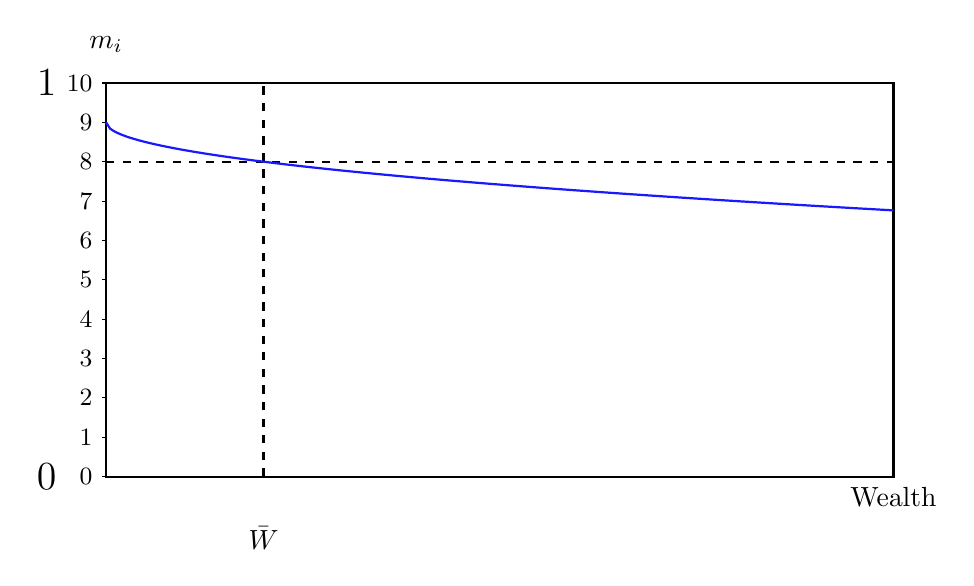
\begin{tikzpicture}[scale=.5]
%\def\bndmax{5}        %https://tex.stackexchange.com/questions/68462/filling-a-complex-region-with-tikz
%\def\bndmin{0.2}
\def\Y{10}  % height of y axis pecent
\def\W{20}  % length  of x axis
\def\Wbar{4}
\def\rbar{8}% this is the prime rate

% %Equation   \[ r_i = (A + .5 \frac{\bar{W}}{W_i})\omega\]
   % \def\Wmin{.63}  %This sets the lower limit fo the 
    \def\Wmin{(\B*\Wbar)/(\Y/\rbar-\A)} %function to keep in in bounds
	
 \tikzset{func/.style={thick,color=blue!90}}	

 \draw [thick](\W,\Y)-- (0,\Y)node[left=.5cm]{\Large$1$}node[above=.25cm]{$m_i$} -- (0,0)node[left=.5cm]{\Large$0$}--(\W,0)node[below]{Wealth}--cycle;  	% Axes box
 
 \draw [dashed, thick] (0,\rbar) -- (\W,\rbar);  	% Axes
\draw [thick,dashed] ( \Wbar,0)node[below=.5cm]{$\bar{W}$} -- (\Wbar,\Y);  	% Axes

\foreach \yi in {0,...,\Y} \draw (0,\yi)--(-.1,\yi)node[left]{\small$\yi$};
%\foreach \yi in {0,2,4,6,8,10} \draw (0,\yi)--(-.1,\yi));
%node[left]{\small$\yi$};
%\foreach \yi in {0,2,4,6,8,10}node at (-.1,yi) {{10*yi}} ;
\draw[func,domain=0:\W] plot [samples=200] (\x,(9-\x^.5/2);

 \end{tikzpicture}
\caption{Individual borrowing ratio $m_i$ as a function of wealth (in tenths)}
 \label{Fig:Borrowingratio}
\end{figure}


\subsubsection{Individualized borrowing rates}\label{SS:BorowingRate}
 
 
 $r_i$ depends on relative income and assets, as well as base interest rates. % compared to others. 
 The median after-tax income of Canadian families and unattached individuals was \$66,800 in 2020 according to Statistics Canada's %\href{https://www150.statcan.gc.ca/n1/daily-quotidien/220323/dq220323a-eng.htm}{Canadian Income Survey, 2020}.  \href{https://www150.statcan.gc.ca/t1/tbl1/en/tv.action?pid=1110005501}
 Data released in 2020 by Statistics Canada indicates that the top 1\% of Canadians made, on average, around \$512,000 in a single year \cite{stats-can-canadian-incomes}. % \href{https://www150.statcan.gc.ca/n1/daily-quotidien/201222/dq201222b-eng.htm}{Survey of Financial Security, 2019}.

 A study by Statistics Canada found that the typical Canadian household now has a median net worth of \$329,900, while the average net worth in Canada is \$738,200 \cite{stats-can-median-net-worth}.  %\href{https://www150.statcan.gc.ca/t1/tbl1/en/tv.action?pid=1110005501}{High income tax filers in Canada}

\subsubsection{Computing the income constraint on interest rates}\label{SS:YWealthConstraint}
$r_i$

In our model, we  tie the individual cost of capital,  $r_i$ for agent $i$, to a prime rate, $\bar r$ or the bank's target rate, $r^{target}$, prime plus 1\%, say. and to individual wealth. Figures~\ref{Fig:Borrowingrate1} and ref{Fig:Borrowingrate1} illustrate a couple of possible  cost-of-borrowing models roughly consistent  with the stylized facts about lenders. 

\begin{align}
 r_i =  &  \left(A + B \frac{\bar{W}}{W_i}\right) \bar r       \label{eq:incomeandr1}  \\
 r_i =  &  \left(\bar r - A + B *\frac{\bar W}{W_i - C}\right) \label{eq:incomeandr2}  \\
\end{align}
Where $\Bar{W}$ is mean wealth and $W_i$ is individual wealth. In Equation~\ref{eq:incomeandr2},  A determines y-shift, B, the scale, and C the  x-shift for the curve.


\begin{figure}
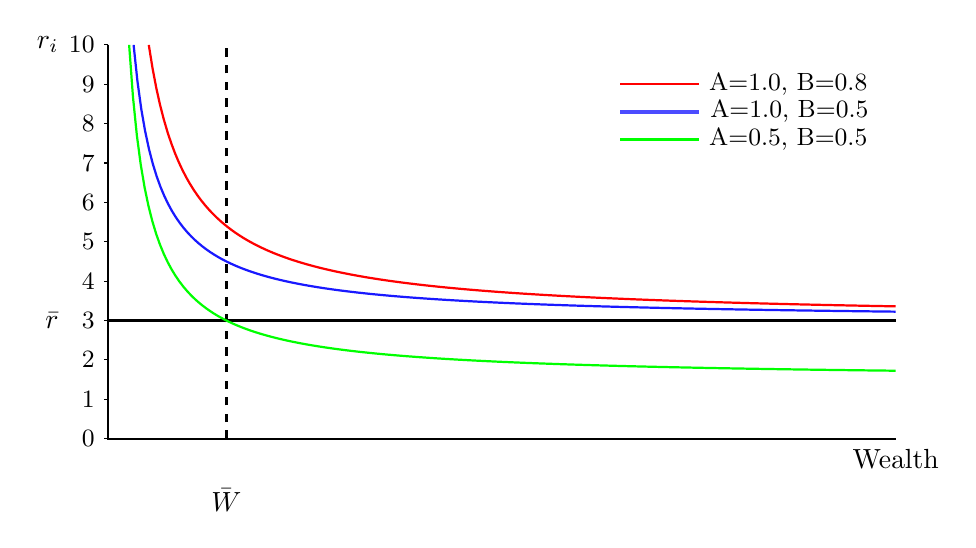
\begin{tikzpicture}[scale=.5]
%\def\bndmax{5} % https://tex.stackexchange.com/questions/68462/filling-a-complex-region-with-tikz
%\def\bndmin{0.2}
\def \Y {10}    % height of y axis as a pecent
\def \W {20}    % length  of x axis
\def \Wbar {3}  % mean wealth
\def \rbar {3}  % the prime rate 

% Equation   \[ r_i = (A + .5 \frac{\bar{W}}{W_i})\omega\]
\def \Wmin{.63}  %This sets the lower limit fo the 
\def \Wmin{(\B*\Wbar)/(\Y/\rbar-\A)} %function to keep in in bounds
\tikzset{func/.style={thick}}	

% Axes
\draw [thick] (0,\Y)node[left=.5cm]{$r_i$} -- (0,0)--(\W,0)node[below]{Wealth};  
\foreach \yi in {0,...,\Y} \draw (0,\yi)--(-.1,\yi)node[left]{\small$\yi$};
\draw [thick] (0,\rbar)node[left=.5cm]{$\bar r$} -- (\W,\rbar);  	% Axes
\draw [thick,dashed] ( \Wbar,0)node[below=.5cm]{$\bar{W}$} -- (\Wbar,\Y);  	% 

\def \A {1.0}  \def \B {0.5} %BLUE
\draw[func,domain=\Wmin:\W, color=blue!90] plot [samples=200] (\x,{(\A+\B*\Wbar/\x)*\rbar});
\draw [ultra thick, color=blue!70 ](13, 8.3)--(15,8.3)node [right, black] {\small A=\A,\ B=\B};

\def \A {0.5} 
\def \B {0.5} % GREEN
\draw[func,domain=\Wmin:\W, color=green] plot [samples=200] (\x,{(\A+\B*\Wbar/\x)*\rbar});
\draw [thick,  color=green](13, 7.6)--(15,7.6)node [right, black] {\small A=\A, B=\B};

\def \A {1.0}  \def \B {0.8} % RED
\draw[func,domain=\Wmin:\W, red] plot [samples=200] (\x,{(\A+\B*\Wbar/\x)*\rbar});
\draw [thick,  color=red](13, 9)--(15,9)node [right, black] {\small A=\A,\ B=\B};
% KEY
\end{tikzpicture}
\caption{Individual borrowing cost as a function of wealth}
\label{Fig:Borrowingrate1}
\end{figure}


\begin{figure}
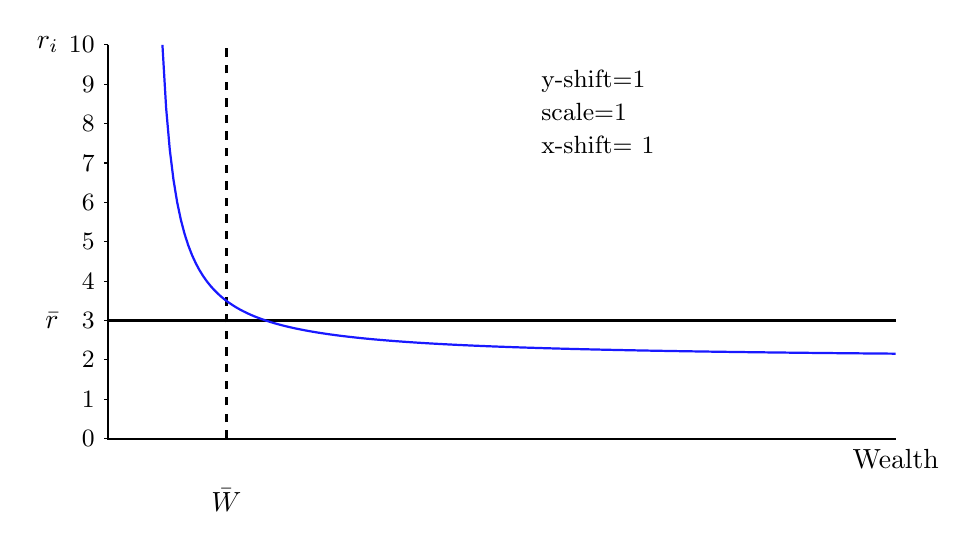
\begin{tikzpicture}[scale=.5]
%\def\bndmax{5}        %https://tex.stackexchange.com/questions/68462/filling-a-complex-region-with-tikz
%\def\bndmin{0.2}
\def \Y {10}  % height of y axis pecent
\def \W {20}  % length  of x axis
\def \Wbar {3} % meam wealth
\def \rbar {3}% this is the prime rate 

%\def \Wmin{(\B*\Wbar)/(\Y/\rbar-\A)} %function to keep in in bounds
\tikzset{func/.style={thick}}	
	% Axes
\draw [thick] (0,\Y)node[left=.5cm]{$r_i$} -- (0,0)--(\W,0)node[below]{Wealth};  
\foreach \yi in {0,...,\Y} \draw (0,\yi)--(-.1,\yi)node[left]{\small$\yi$};
\draw [thick] (0,\rbar)node[left=.5cm]{$\bar r$} -- (\W,\rbar);  	% Axes
\draw [thick,dashed] ( \Wbar,0)node[below=.5cm]{$\bar{W}$} -- (\Wbar,\Y);  	% 

\def \A {1} %vertical shift aroung \rbar, the prime rate
 \def \B {1}  % Scales the exponential curveBLUE
 \def \C {1}  %right shift  
% \def \Wmin {.4+\B}  %This sets the lower limit fo the 
\def \Wmin {(\B*\Wbar)/(\Y-\rbar+\A) +\C} %function to keep in in bounds

\draw[func,domain=\Wmin:\W, color=blue!90] plot [samples=200] (\x,{\rbar-\A+\B*\Wbar/(\x-\C))});
\node  [align=left, text width =2cm ] at (13, 8.3) {\small y-shift=\A \newline scale=\B \newline x-shift= \C};

 \end{tikzpicture}
\caption{Individual borrowing cost as a function of wealth II}
\label{Fig:Borrowingrate2}
\end{figure}

The rates $\delta,\ \sigma,$ and $r$ depend on the period, $T$. 

\subsection{Incorporating growth and discounting}
%We need a time period T for calculations. For use in any calculation, 

With a price-growth rate of $\dot P$ per year, the growth over $T$ years is $(1+\dot P)^T$, and  %and a 5 year mortgage period, 
the expected price at the end of the period is:

\[P_M^{Te}=P_0(1+\dot P)^T\]

If, for example price growth is 10\%, $\dot P= 0.1$, the {capital gain}, or growth, over a 5-year mortgage term is 0.61051 $\approx$ 60\% of the original price, $P_0$.

If we want the compounded interest rate person $i$ the term T,
\[r_i^T=(1+r_i)^T\]
% This is the value we use in equation~\ref{EqBidPrice}.

If person $i$  discounts at a discount rate $r^\delta$, the present value of a receipt at time $t$ is calculated by using the \textbf{discount factor} $\delta_i^T$.

\[\delta_i^T= \left( \frac{1}{1+r_\delta} \right)^T \]
%\[\delta_i^T= \sum_{\tau=0}^{\tau=T}\left( \frac{1}{1+r_\delta} \right)^\tau \]
 
These can be combined into a function %\delta that  gives a single discounting factor  for a value  like future price that is both growing and being discounted over several (T) periods:
\[ PDV(P_M^{Te})=P_0\left( \frac{1+\dot P}{1+r_\delta} \right)^T \]
This PDV function specifically combines any expected rent increase, the individual's discount rate and the mortgage term into a single operation.

\subsection{Mortgage availability}
For home loans, many personal finance experts recommend total housing costs account for less than 28\% of your \textbf{gross} household income, This gives us an \textbf{income-based  mortgage maximum} of \[M^{max}_Yi = \frac{0.28*(\omega+w)}{r_i}\] It is the maximum the bank will let you pay.

We assume $r_i$ is based on the individual's assets, on relative wealth. Where is it calculated for the householder or the bank?

We get a \textbf{price-based mortgage maximum} \[M^{max}_P = 0.8P_0\] where $P_0$ is the actual sale price. This is based on the maximum amount of risk that the bank is willing to take on. ($P_0$  will not always be the same as the asking price or the warranted price.)


\section{TO SORT: Miscellaneous calculations about rates over time}


$delta(0)=1$  for funds received now

Lets calculate $S$, $\delta$ at time infinity:
*** Why?

\[\delta(t)=\left(\frac{1}{1+r}\right)^t\]



\begin{align}
delta (1)   &= 1/(1+r) \\
delta (t)   &= (1/(1+r))^t \\
delta (\infty)   &= \sum_0^\infty\left(1/(1+r)\right)^t\\ 
Let\ a=1/(1+r)&<1\\
delta (\infty)   &= \sum_0^\infty a^t\\ 
S               &= \sum_0^\infty a^t\\ 
               &= 1+a+a^2+a^3+a^4 \dots\\ 
S-aS             &= 1\\ 
S             &= 1/(1-a)\\ 
S             &= \frac{1}{1-\frac{1}{1+r}}\\ % subing r back in for a 
             &= \frac{1}{1-\frac{1}{1+r}}\\ 
             &= \frac{1}{\frac{1+r-1}{1+r}}\\ 
              &= \frac{1}{\frac{r}{1+r}}\\ 
             &= \frac{1+r}{r}
\end{align}
This is the case where you get paid at the beginning of the first period. Rent might be paid in advance for each month. .

For  the case where you get pay at the end of the first period. Interest on a loan  might be paid this way.  summing from t=1 this time, we get $S-aS =a$, and $S = a/(1-a)= \frac{1}{r}$. 

 

%\[\delta(t)= \delta(1)^t =\left(\frac{1}{1+r}\right)^t\]

Finally, we need an expression for the sum of a finite  series to T.  Doing the derivation to check my logic, notice that  omega, psi, c  and a are constants that can be factored out in the following,(\textbf{THIS IS THE WRONG PROPERTY VALUE}
%\[\left(c*\omega + c*a*\psi \right) ->c\left(\omega-trans\ d + a\psi \right)\]
\begin{align}%
    tax&= \sum_{t=0}^{T-1} \delta(t) \left(c*\omega + c*a*\psi \right)\\
        &= c(\omega + a\psi)\sum_{t=0}^T  \delta_t\\
        &= c(\omega + a\psi)(\delta_1+\delta_2 \dots \delta_T)\\
        &= c(\omega + a\psi) \left(\sum_0^\infty \delta_t-\sum_{T}^\infty \delta_t\right)\\
        &= c(\omega + a\psi) \left(\frac{1+r}{r}  - \left(\frac{1}{1+r}\right)^{T+1} \left(\frac{1+r}{r} \right) \right)\\
        &= c(\omega + a\psi) \frac{1+r}{r}\left(1  - \left(\frac{1}{1+r}\right)^{T+1} \right)
%      &=& c(\omega + a\psi)\delta_T\\
\end{align}








\section{Table of Parameter Values}

\renewcommand{\arraystretch}{1.5}
\begin{tabular}{rlrr}\
Symbol         & Name                                 & Value      & Formula  \\ \hline
$a$ replace    & Share of $\psi$ for land and building &   0.3         & \\
$b$ replace    & Share of $\psi$ for maintenance       &   0.2         & \\
$tau$ replace  & Property tax rate &  e.g 1.6\% = 16 mills             & \\
$c$       & Transportation cost & \\
$T$       & Period & 5 years      \\
$r$       & Individual interest rate & 0.05 \\
$\omega$  & Locational rent & 0.012  \\
$\psi$    & Subsistence wage & 10000 \\
$a$       & Share of subsistence wage for land and building & 1.0 \\
$\tau$       & Tax share & \\

--        &  & \\
$m_i$          & Individual borrowing-ratio           & 0.75-0.85  & $M/P^{ask?}$ \\
$M^{max}_Yi$.  & Maximum mortgage based on income     &            & $\frac{0.28(\omega+w)}{r_i}$ \\
 $M^{max}_P$   & Maximum mortgage based on the price  &            & $0.8*P_0$ \\
$IS$           & Income share for housing debt        & 0.25-0.35  & Missing? \\
$\rho$         & Rent ratio                           &            & $\frac{\omega-tau*d_i}{P_0}$ \\
$\kappa $      & Operations ratio                     & 0.1-0.3    & e.g. $ 0.2\frac{\omega-tau*d_i}{P_0}$ \\
$\sigma$       & Tax ratio                            & 0.25-0.35  & e.g. $ 0.3\frac{\omega-tau*d_i}{P_0}$ \\
$\dot P $      & Price growth                         & []         & $\frac{P_t-P_{t-1}}{P_{t-1}}$\\
% $P^T_e$        & Expected price in T years            &            & $P_0(1+\dot P)^T$ \\ % *** WAS $P^e_T$ 
$r_i^\delta$   & Individual discount rate             &            & To assign \\
$\bar r$       & Prime interest rate                  &            & \\
$r_i$          & Individual borrowing-rate            &            & \\
$r^{target}$   & Target interest rate                 &            & $\bar r + margin$ \\
$\delta_i$     & Discount factor for T                &            & $\left(\frac{1}{1+r_i^\delta}\right)^T$ \\


\end{tabular}
\renewcommand{\arraystretch}{1.0}




discount rate vs discount factor

% delta(0)=1  delta (1)= 1/(1+r) 
\[\delta(t)=\left(\frac{1}{1+r}\right)^t\]
    $delta_T=  (1/(1+r))^T$   at T years
    eg r=.05  T=5  delta5 =  $(1/(1+.05))^5 = 0.7835262$


\section{Notation Table}
% \section{Notation for Urban and Production Sectors}
\begin{longtable}{lp{10cm}}
\caption{Notation}                       \\

\hline           &  \textbf{Productivity} \\ \hline
$K$              &  Capital               \\ 
% $L$            &  Labour                \\
$N$              &  Population, equals labour \\ %, $L$                     
$Y=N^\gamma K^{\alpha }N^{\beta }$  &  Output \\ %Urban output            \\
$\alpha$         &  Elasticity of output with respect to capital          \\
$\beta$          &  Elasticity of output with respect to labour           \\ % vs effective labour
$\gamma$         &  Elasticity of agglomeration with respect to labour    \\ % , $\Lambda(n)$, for illustration \\

% $L$              &  Labour supply \\ %the number of workers, which, in the standard circular city model, equals the number of lots of size $s$  when workers live on identical individual lots. % Unless $d^{max}>d^*$ v  \frac{\pi}{s}(\frac{w}{{c}})^2 =
% $n_i$  &  Number of workers employed by firm $i$ \\
% n=\sum_i n_i$  &  Number of workers, the urban population in the model \\
% $\#f=\frac{n}{n_i}$&number of identical firms \\ %not used
% $f$  &  Number of firms =1 \\
% $n =f n_i$  &  Aggregate labour \\
% $\Lambda(n)$    &  Labour-augmenting agglomeration effect \\
% $n^\gamma$ & The labour-augmenting agglomeration effect,  modelled as an exponential function of the number of people \\
% $\Lambda(n)n_i$ &  Effective labour for firm $i$ \\
% $\Lambda'=\die{\Lambda(n)}{n} $ & Derivative of the labour-augmenting agglomeration effect\\

%%$Y_i=K_i^{\alpha }(\Lambda(n)n_i)^{\beta }$  &  Urban firm $i$'s output \\

%%$Y=\frac{n}{n_i}K_i^{\alpha }(\Lambda(\sum_i n_i)n_i)^{\beta }$  &  Aggregate output of all firms in the city \\
% $\die{Y}{n}=\beta\frac{1}{n} Y  \left( 1+ \frac{n\Lambda'}{\Lambda} \right)$  &  Social marginal product of labour \\
% $Y_i=K_i^{\alpha }(\Lambda(n)n_i)^{\beta }$    &  Urban firm $i$'s output \\
% $\die{Y_i}{K_i}	=\alpha \frac{1}{K_i} Y_i $  & Marginal product of capital for firm $i$ \\
% $\die{Y_i}{n_i}	=  \beta\frac{1}{n_i} Y_i $  &  Marginal product of labour for firm $i$ \\
%%$\eta=\frac{n_i\Lambda'}{\Lambda}$  &   Marginal agglomeration effect on a firm's output of increasing it's own labour stock \\
% \hline
	% &\textbf{Amenity}\\ \hline
% $A(d, n)$   &  Agglomeration amenity          \\

\hline           &  \textbf{Labour market}      \\ \hline %and urban stucture??
$\psi$           &  Rural wage                  \\  
$\omega$         &  Urban wage premium          \\
${c}$            &  Transportation cost per unit distance \\ % Was $\tau$, and $trans$. Considered $\gamma, \xi, \zeta$.
$d$              &  Distance from city centre   \\
$d^* = w/{c}$    &  City extent \\ %, the maximum distance commuters will travel \\ % Maximum distance commuters will travel \\ % to get the wage premium \\
% $\mathcal{R} = w-{c} d$ &  Rent at distance $d$ \\ 
% $\zeta$          &  Population density at distance $d$     \\
% $s$              &  Lot size      \\
% $\psi$  &  ?Per-period cost of a unit of productive capital \\
% $\omega + \psi$  &  Urban wage including rural wage \\ %***
% $\textit{t}$ & {\color{red}transportation cost per km} \\%use   c?
% $w^n=w-{c} d$ & Wage  premium net of transportation costs \\
%% $\Omega=\frac{w+\psi}{\psi}$  &  Ratio of the urban wage to the  cost of capital \\
%% $\Pi$	   &  Profit \\
%% $ER$	   &  Excess return to capital \\ 
% \hline &\textbf{Spatial structure in the circular city} \\ \hline		
%% $d^{max} = w/{c}$  &  Maximum distance commuters at which residents enjoy the urban amenity \\
%% $d^{**} = max(d^*, d^{max})$  &  radius of the city \\
%% $U$                     &  Worker utility **\\ %, a function of location and prices \\
%% $U^{urban}=U^{rural} $  &  Migration equilibrium assumption ** \\
% \hline & \textbf{Labour market} \\ 

\hline           & \textbf{Financial market}             \\ \hline
$P_W$            &  Warranted price for a property       \\
$P_B$            &  Bid price                            \\ % was P^{bid}
$P_A$            &  Asking price                         \\
$P_M$            &  Realized market price                \\
$P_M^e$          &  Expected market price                \\
% $P$            &  Price of a property                  \\ 
% $\dot P$       &  Rate of price growth              \\ % was $\dot p$  
$\mathcal{C}$    &  Capital gains                     \\ % was C
$\mathcal{C}_N$  &  Net capital gain, $C -$ net rent  \\
$M$              &  Mortgage                          \\ 
$m$              &  Mortgage share                    \\ 
$\mathcal{R}$    &  Rent                              \\
$\mathcal{R}_N$  &  Net rent                          \\
${R}^w_N$        &  Warranted rent                    \\
$\rho$           &  Rent ratio                        \\
$\phi$           &  \Gls{rent share}                  \\
$\mathcal{O}$    &  Operational costs                 \\
$\theta$         &  Operations ratio                  \\ % was $\kappa$
$\mathcal{T}$    &  Taxes                             \\ % was $\Sigma, \Xi$  
$\tau$           &  Property tax share                \\ % was t then $\sigma, \xi$
$r$              &  Interest rate                     \\
$\delta$         &  \Gls{discount factor}             \\
% $W$            &  Wealth                            \\
% $\psi$         &  Fraction with rent/operating costs\\
$t$              &  Time                              \\
$T$              &  Time period                       \\

$a$ replace      &  Share of subsistence wage  used for land and building \\
$b$ replace      &  Share of share of subsistence wage used for maintaining home \\ % A cost. Includes water, electricity, heat? 
$tau$            &  Annual tax rate on rent and home \\ % Was $c$

\hline
\color{black}
\end{longtable}  

\newpage

\begin{longtable}{lp{10cm}}
\caption{Rent}                                                            \\
\hline
$\omega-{c} d$                &  Warranted (economic) rent                \\
$\mathcal{R}=\omega-{c} d$    &  Equilibrium rent payment of tenant       \\
PDV                           &  Present discounted value                 \\  
$\mathcal{R}^T$               &  PDV of rent collected over period $T$    \\ 
$\mathcal{R}^T_N=(1-\kappa-\sigma)\mathcal{R}^T$  &  PDV of net rent collected over period $T$ \\
\hline
\end{longtable}

\begin{longtable}{lp{10cm}}
\caption{Bidding Mechanism Notation}                                          \\
\hline
$\mathcal{R}_N$  &  Net rent                                                  \\ % was NR
% $P_0$            &  Purchase price for a property                             \\
% $P^T_e$          &  Expected price at the end of period $T$                   \\
$\bar r$         &  Prime interest rate                                       \\
$r^{target}$     &  Investor or banks target interest rate, $\bar r + margin$ \\
$r_i$            &  Agent $i$'s personal borrowing rate                       \\
$r_i^T$          &  Agent $i$ interest rate compounded over a period $T$      \\
$r_i^{disc}$     &  Agent $i$'s subjective discount rate (which may equal $r_i$) \\
$r_\delta$       &  Discount rate                                             \\ % was $discr_i$
$\delta_i^T$     &  Discount factor for agent $i$ over period $T$             \\
$m^W$            &  Wealth-based share of home price a worker can mortgage    \\ % $= m_i(W_i)$
$m^\omega$       &  Income-based share of home price a worker can mortgage    \\ % IS_i   IS_i(\omega+\psi)$$
$m_i = min(m^W_i, m^\omega_i)$  & Mortgage, the share of home price worker $i$ can mortgage \\

\hline
\color{black}
\end{longtable}  

Notation: 
Agent counts and indices are subscripts.
Values related to time are superscripts, time as a continuous 
variable is small, a period is capitalized e.g. the period $T$ of some number of years. 
In general values are capitals, rates are small letters.

It might be better to use the subscript $m$ for `market'.  for warranted rents

\section{Additional Assumptions}
\begin{enumerate}
\item There is full employment, no frictional unemployment, and no labour adjustment costs.
\item Firms set output and factor inputs to maximize profits, so factors are paid the value of their marginal private product
\item Demand for output is perfectly elastic (constant price = 1)
\end{enumerate}


Rural producers pay a wage $\psi$. this covers a standard house, lot, entertainment, diet and consumption pattern. We  choose units so that per-period cost of a unit of productive capital is also $\psi$